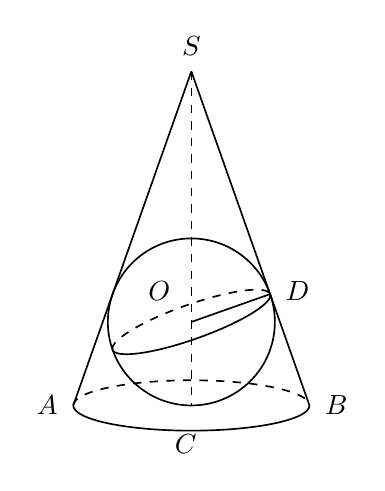
\begin{tikzpicture}[x=1cm,y=1cm,font=\normalsize,line width=.6pt]
\coordinate (S) at (0.0000000000,4.2426406871);
\coordinate (C) at (0,0);
\coordinate (A) at (-1.5,0);
\coordinate (B) at (1.5,0);
\coordinate (O) at (0.0000000000,1.0606601718);
\coordinate (D) at (1.0000000000,1.4142135624);
% cone sides
\draw[solid] (S) -- (A);
\draw[solid] (S) -- (B);
% base ellipse: front solid, back dashed
\draw[solid] (A) arc [x radius=1.5,y radius=0.32,start angle=180,end angle=360];
\draw[dashed] (A) arc [x radius=1.5,y radius=0.32,start angle=180,end angle=0];
% axis
\draw[dashed] (S) -- (C);
% inscribed circle (axis section circle)
\draw[solid] (O) circle [radius=1.060660171780];
\begin{scope}[shift={(0,1.0606601718)},rotate=19.4712206345]
\draw (-1.0606601718,0) arc (180:360:1.0606601718 and .22);
\draw[dashed] (-1.0606601718,0) arc (180:0:1.0606601718 and .22);
\end{scope}
% radius OD
\draw[solid] (O) -- (D);
\node[above,yshift=2pt] at (S) {$S$};
\node[left,xshift=-2pt] at (A) {$A$};
\node[right,xshift=2pt] at (B) {$B$};
\node[below,yshift=-7pt,xshift=-2pt] at (C) {$C$};
\node[above left=4pt] at (O) {$O$};
\node[right,xshift=2pt,yshift=1.0pt] at (D) {$D$};
\end{tikzpicture}
